\chapter{Výběr a návrh elektroniky}
Výběr elektronických součástek probíhal dle jejich parametrů, využití, dostupnosti a~ceny. Nejdříve byla vybrána bezdrátová technologie a mikrokontrolér a v~závislosti 
na tom vše ostatní. 

\section{Bezdrátová technologie}
Ke komunikaci Semaforů mezi sebou byla zvolena technologie LoRa a pro bezdrátovou konfiguraci Semaforů byla zvolena technologie WiFi. 

\subsection{LoRa}
 Tato technologie byla zvolena především kvůli komunikačnímu dosahu. Jedná se sice o~dražší technologii, 
ale na tolik, aby ji nebylo možné v~tomto zařízení použít. Táborové hry se většinou hrají na loukách, které mají rozlohu několik stovek metrů čtverečných. LoRa je jedinou
dostupnou technologií, která na tyto vzdálenosti spolehlivě komunikuje. Bezdrátové propojení Semaforů bude použito pro posílání informací o~aktuálně svítící barvě, či 
stisku tlačítka v~závislosti na hře, která se aktuálně hraje. U~některých her například může být žádoucí, aby po přepínání nesvítily všechny Semafory stejnou barvou 
a díky této komunikaci bude moci být takovým stavům zabráněno. 

Byl vybrán bezdrátový LoRa modul E22-900T22D od firmy EBYTE. Tento modul komunikuje s mikrokontrolérem pomocí UART sběrnice \cite{LoRa_ebyte}. Jeho napájecí napětí je od 
2,1 V do 5,5 V a komunikační napětí je 3,3 V \cite{LoRa_ebyte}. Rozsah komunikačních frekvencí bezdrátového modulu E22-900T22D je 850,125 MHz až 930,125 MHz a ve výchozím 
stavu je nastavena na 868,125 MHz \cite{LoRa_ebyte}. Toto je frekvence, na které je v ČR povoleno komunikovat a to s maximálním vyzařovaným výkonem 25 mW \cite{CTU}. 
Maximální povolený klíčovací poměr je 1 \% \cite{CTU}. %klíčovací poměr = max duty cycle 
V běžném režimu je spotřeba přibližně 151 mA a v režimu spánku 2 $\mu$A \cite{LoRa_ebyte}. Tento bezdrátový modul má externě připojitelnou anténu typu SMA-K s 50 $\Omega$ 
impedancí \cite{LoRa_ebyte}.

LoRa modul E22-900T22D je připojen k mikrokontroléru pomocí komunikačních pinů RX a TX sběrnice UART. Napájecí napětí tohoto modulu je spínáno mikrokontrolérem, aby jej 
šlo v případě nůzkého napětí baterie odpojit. Pin AUX slouží k indikaci funkčního stavu modulu. Při specifických aplikacích slouží pro probuzení externího mikrokontroléru. 
Pin AUX není v této aplikaci využíván, a proto není nikam připojen. Pomocí pinů M0 a M1 lze přepínat bezdrátový modul do různých režimů. Pokud jsou oba piny v logické 1, 
tak je modul přepnut do režimu spánku \cite{LoRa_ebyte}. Pokud jsou oba piny v logické 0, tak je modul v normálním režimu \cite{LoRa_ebyte}. V této aplikaci je modul 
provozován pouze v normálním režimu, a proto jsou piny M0 a M1 připojeny k signálu GND. 

\begin{table}[!h]
  \caption[Konfigurační piny LoRa modulu E22-900T22D]{Konfigurační piny LoRa modulu E22-900T22D \cite{LoRa_ebyte}}
  \begin{center}
  	\small
	  \begin{tabular}{|c|c|c|c|}
	    \hline
	    \textbf{M0}	& \textbf{M1}	& \textbf{Mód} & \textbf{Popis} \\
	    \hline
	    0	& 0 & Normální & UART a bezdrátový kanál otevřený, \\ 
      & & &transparentní přenos zapnutý \\ 
	    \hline
	    0	& 1 & Režim WOR & Lze definovat jako vysílač WOR \\
      & & & a přijímač WOR \\ 
	    \hline
	    1 & 0 & Konfigurační mód & Přistup k registru přes sériový port \\
      & & & a ovládání pacovního stavu \\
	    \hline
      1 & 1 & Režim hlubokého & Režim spánku \\
      & & spánku & \\
	    \hline
	  \end{tabular}
  \end{center}
\end{table}

%obrazek se zapojenim LoRa modulu

\subsection{WiFi}
K~propojení Semaforu s~telefonem a dalšími zařízeními byla vybrána technologie WiFi. Jedná se o~rozšířenou technologii, která je v~telefonech a noteboocích zabudovaná. 
Propojení bude tedy jednoduché a nastavovat hry se mohou na webové stránce, kde bude seznam her, které Semafor umí. U~jednotlivých her se poté budou moci nastavovat 
další parametry. Po nastavení se konfigurace pošle do Semaforu. 

%více rozepsat info o WiFi

\section{Mikrokontrolér}
WiFi modul obsahuje jako jediný mikrokontrolér od firmy Espressif z~řady ESP32. Konkrétně jde o~typ ESP32-C3-MINI-1, dále již jen ESP32-C3. Je také nabízen za cenu, která 
je v~porovnání s~ostatními nízká a v~porovnání s~nabízenými parametry bezkonkurenční. Pro zařízení Semaforu je také se svým počtem periferií dostačující. ESP32-C3 má 
384 kB ROM a 4 MB flash paměti \cite{ESP_C3_dtsh}. Dále obsahuje WiFi modul pracující na frekvenci 2,4 GHz a Bluetooth \cite{ESP_C3_dtsh}. ESP32-C3 obsahuje mnoho periferií
jako je SPI, UART, $I^2C$, USB a další \cite{ESP_C3_dtsh}. Mikrokontrolér má vyvedeno 13 GPIO pinů, které je možno softwarově nastavit jako vstupní nebo výstupní. Tyto piny
slouží pro připojení senzorů, díky kterým je zprostředkována komunikace mezi mikrokontrolérem a okolním světem. V~mikrokontroléru je také zabudován krystal s~vlastní frekvencí 
40 MHz a v~rámci pouzdra je také anténa pro WiFi \cite{ESP_C3_dtsh}.

Rozsah napájecího napětí je 3~až 3,6~V~\cite{ESP_C3_dtsh}. Jeho maximální proudový odběr je 0,5~A~\cite{ESP_C3_dtsh}. Mikrokontrolér ESP32-C3 garantuje pracovní teplotu 
od -45~°C až do 85~°C \cite{ESP_C3_dtsh}.

\begin{figure}[!h]
  \begin{center}
    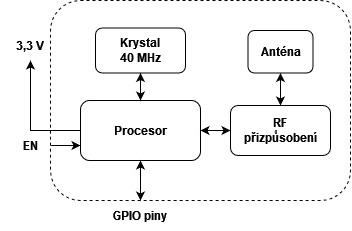
\includegraphics[scale=0.8]{obrazky/blokove_schema_MCU.jpg}
  \end{center}
  \caption[Blokové schéma mikrokontroléru ESP32-C3]{Blokové schéma mikrokontroléru ESP32-C3 \cite{ESP_C3_dtsh}.}
\end{figure}

K~pinu 3V3, který slouží pro připojení napájecího napětí jsou také připojeny kondenzátory o~hodnotě 10 $\mu$F a 100 nF dle doporučení z~dokumentace \cite{ESP_C3_dtsh}. Tyto 
kondenzátory slouží pro filtraci napájecího napětí, aby bylo vyfiltrováno případné rušení o~různých frekvencích.

Pin EN slouží pro povolení funkce mikrokontroléru. Tento pin nesmí zůstat nezapojený, tzv. floating. Jeho zapojení je převzato z~dokumentace, tj. pullup rezistor o~hodnotě 
10 k$\Omega$ a ke GND je připojen přes kondenzátor o~hodnotě 1 $\mu$F \cite{ESP_C3_dtsh}.

\begin{figure}[!h]
  \begin{center}
    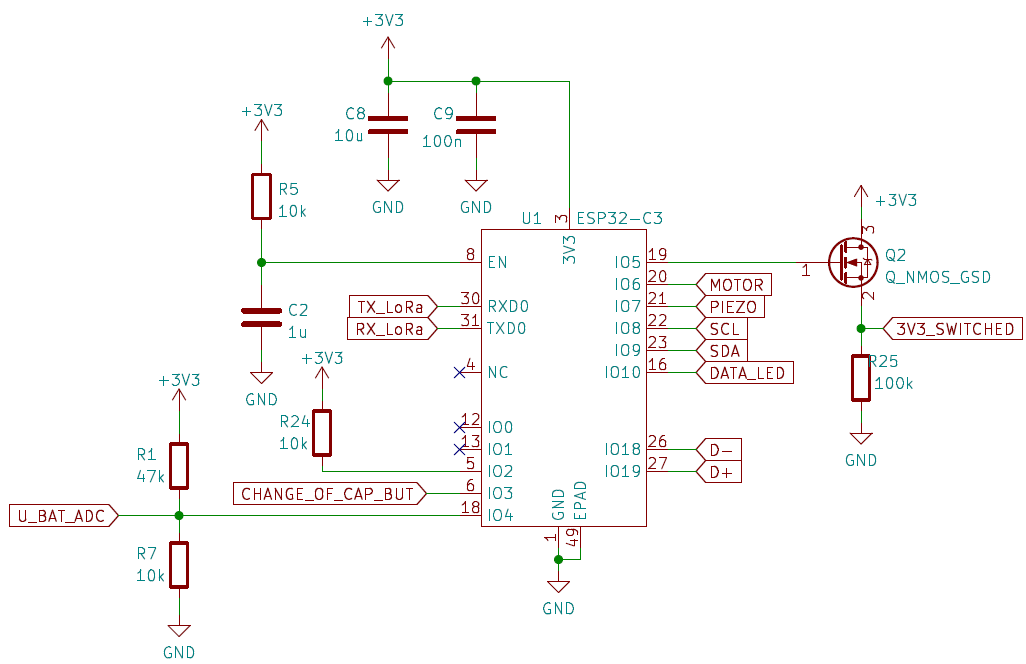
\includegraphics[scale=0.5]{obrazky/ESP32-C3.png}
  \end{center}
  \caption[Schéma zapojení mikrokontroléru ESP32-C3]{Schéma zapojení mikrokontroléru ESP32-C3.}
\end{figure}

ESP32-C3 má konfigurační piny, které slouží při restartu pro určení, odkud bude načten program pro mikrokontrolér. Tyto piny musí být při restartu v~daném nastavení. 
Konfiguračními piny jsou GPIO2, GPIO8 a GPIO9. Piny GPIO8 a GPIO9 nesmí být nikdy nastaveny současně do logické nuly. 

\begin{table}[!h]
  \caption[Konfigurační piny ESP32-C3]{Konfigurační piny ESP32-C3 \cite{ESP_C3_dtsh}}
  \begin{center}
  	\small
	  \begin{tabular}{|c|c|c|c|}
	    \hline
	    \textbf{Pin}	& \textbf{Výchozí}	& \textbf{Načtení programu} & \textbf{Načtení programu} \\
      \textbf{}	& \textbf{}	& \textbf{z~flash paměti} & \textbf{z~bootloaderu} \\
	    \hline
	    \textbf{GPIO2}	& Není dostupný & 1 & 1 \\ 
	    \hline
	    \textbf{GPIO8}	& Není dostupný & Nezáleží & 1 \\ 
	    \hline
	    \textbf{GPIO9} & Interní měkký pullup & 1 & 0 \\
	    \hline
	  \end{tabular}
  \end{center}
\end{table}

Protože bude využito programování přes USB piny D+ a D-, tak není zapotřebí načtení z~bootloaderu a je tedy zapotřebí všechny konfigurační piny při restartu připojit do 
logické jedničky. Do logické jedničky lze připojit přes pullup rezistor. Pullup rezistory má sběrnice $I^2C$, takže na GPIO8 a GPIO9 byla připojena právě sběrnice $I^2C$.
Pin GPIO2 nebyl využit pro připojení žádného senzoru, a proto byl připojen přes pullup rezistor o~hodnotě 10 k$\Omega$ k~napájecímu napětí.

\section{Napájení}
Zabudování baterie přináší kompaktnost řešení a pro použití není třeba dalších komponent. Pokud je ale na táboře větší využití, tak se baterie vybije.
Na táborech většinou nebývá k~dispozici připojení k~elektrické síti, a proto je řešením powerbanka. Na Semaforu tedy bude napájecí vstup USB-A pro nabíjení baterií
přímo z~powerbanky bez nutnosti kabelu. Semafor musí být koncipován tak, aby se mohla baterie nabíjet a zároveň, aby při tom byly Semafory funkční.

Při realizaci Semaforu byla tedy zvolena kombinace napájení pomocí baterií i~pomocí powerbanky. Článek baterie LiFePO4 byl vybrán právě kvůli již zmíněným vynikajícím 
vlastnostem. Vybraný mikrokontrolér má napájecí napětí v~rozsahu 3 až 3,6 V~\cite{ESP_C3_dtsh}. Pro funkci mikrokontroléru tedy nebude muset být použit ani 
převodník napětí. 

Napětí na baterii je měřeno pomocí děliče a připojeno na pin GPIO4, který má k~dispozici AD převodník \cite{ESP_C3_dtsh}. V~softwaru bude nastaven útlum na 0 dB, to 
odpovídá rozsahu měřeného napětí od 0 do 700 mV \cite{ESP_C3_tech_ref}.
Proto je napětí z~baterie pomocí rezistorového děliče převedeno na rozsah od 0 do 600 mV. Zde je pomocí AD převodníku napětí na baterii měřeno. Spodní rezistor děliče byl
zvolen o~hodnotě 10 k$\Omega$ a druhý byl dopočítán na hodnotu 50 k$\Omega$ podle maximálního napětí baterií LiFePO4 3,6 V. Nejbližší hodnota rezistoru je 47 k$\Omega$
\cite{rezistorova_rada}. Tomu odpovídá maximální napětí na AD převodníku 0,63 V, což je stále v~možném měřeném rozsahu. 

Při nízkém napětí baterie jsou softwarově odpojovány periferie a senzory od jejich napájecího napětí. Děje se tak pomocí pinu GPIO5, na který je připojen spínací 
tranzistor.

\subsection{Nabíjecí obvod}
Nabíjecí obvody jsou závislé na konkrétním typu baterií, které budou nabíjeny. Vzhledem k~vybranému typu baterií LiFePO4 byly uvažovány pouze komerčně
dostupné integrované obvody, které jsou určeny pro nabíjení tohoto typu baterií. 

Vybraný typ baterií LiFePO4 lze nabíjet pomocí obvodu CN3058E. 

Nabíjecí obvod CN3058E je určen pro nabíjení pouze LiFePO4 baterií a lze jím napájet právě 1 článek těchto baterií \cite{charger_dtsh}. Napájecí napětí tohoto 
nabíjecího čipu se pohybuje mezi 3,8 až 6 V~\cite{charger_dtsh}. Díky tomu lze přímo použít napětí z~USB konektoru. 

Když je nabíjecí obvod odpojen od napájecího napětí, tak přejde do režimu spánku \cite{charger_dtsh}. V~tomto režimu je baterie vybíjena proudem menším než 
3 $\mu$A \cite{charger_dtsh}. Tento proud je oproti klidovým proudům jiných součástek zanedbatelný, a proto nemusí být baterie od nabíjecího obvodu odpojována,
když není nabíjena. 

Nabíjecí obvod CN3058E umí také vyhodnocovat teplotu baterie a v~závislosti na tom přestávat baterii nabíjet \cite{charger_dtsh}. Tato funkce není v~zapojení
Semaforu využita, proto je pin TEMP připojen k~signálu GND \cite{charger_dtsh}.

Tento nabíjecí obvod se vyrábí ve standardizovaném pouzdře SOP8 \cite{charger_dtsh}.

\subsection{Zapojení nabíjecího obvodu}
Rezistor připojený k~pinu ISET slouží pro nastavení hodnoty nabíjecího proudu \cite{charger_dtsh}. V~tomto zapojení byl počítán pro nabíjecí proud 1 A~dle rovnice
z~dokumentace: 
\begin{equation} 
  R_{8}~=~\frac{1218}{I_{CH}}~=~\frac{1218}{1}~=~1,218~k\Omega. 
  \quad \quad \quad \quad \quad \quad \quad \quad \quad \cite{charger_dtsh}
\label{eq:I_CH}
\end{equation}

Z~výpočtu vyplývá, že rezistor by měl mít hodnotu 1,218 k$\Omega$. Nejbližší hodnota z~rezistorové řady E12 je hodnota 1,2 k$\Omega$, proto byl také zvolen rezistor 
o~této hodnotě \cite{rezistorova_rada}. Odpovídá tomu nabíjecí proud 1015 mA, který nebude mít vliv na životnost baterií. 

Vstupní a výstupní kondenzátory slouží pro filtraci zákmitů napájecího napětí a také napětí, kterým je nabíjena baterie. Hodnoty kondenzátorů byly převzaty
z~doporučení z~dokumentace, tj. 4,7 $\mu$F \cite{charger_dtsh}.

Kladný pól nabíjené baterie je připojen na pinu BAT, záporný pól je připojen ke GND. Pin BAT poskytuje nabíjecí proud do baterie a zároveň poskytuje konstantní 
nabíjecí napětí. V~režimu spánku je svodový proud tohoto pinu 3 $\mu$A \cite{charger_dtsh}. 

Pin VIN slouží pro napájení vnitřního obvodu CN3058E. Je na něj přikládáno napájecí napětí z~USB, tedy 5 V. Pokud napájecí napětí klesne na napětí o~10 mV nižší, 
než je napětí na pinu BAT, tak vnitřní obvod přechází do režimu spánku \cite{charger_dtsh}. V~tomto režimu klesá proud pinu BAT na méně než 3 $\mu$A \cite{charger_dtsh}.

Tento nabíjecí obvod má možnost indikace nabíjení baterií a dokončení nabíjení. Tato indikace je realizována pomocí 2 LED připojených přes pullup rezistor. Hodnota
pullup rezistoru byla převzata z~doporučení z~dokumentace, tj. 330 $\Omega$. Červená LED indikuje nabíjení baterií a je připojena na pin /CHRG a zelená LED indikuje 
dokončené nabíjení a je připojena na pin /DONE. Obě LED jsou k~pinům nabíjecího čipu připojeny katodou. 

Obvod CN3058E může také měřit teplotu na nabíjené baterii. Slouží k~tomu vstupní pin TEMP. Měření probíhá pomocí odporového děliče, jehož střed je připojen na snímač 
teploty. Tento snímač je připojen na baterii. Pokud je napětí na pinu TEMP nižší než 45 \% nebo vyšší než 80 \% úrovně napájecího napětí, tak je indikována moc nízká
nebo moc vysoká teplota baterie a nabíjení je zastaveno \cite{charger_dtsh}. Jinak nabíjení pokračuje. Uzemněním pinu TEMP je funkce měření teploty deaktivována 
\cite{charger_dtsh}. V~této práci není měření teploty baterií využíváno, a proto je pin TEMP připojen ke GND. 

\begin{figure}[!h]
  \begin{center}
    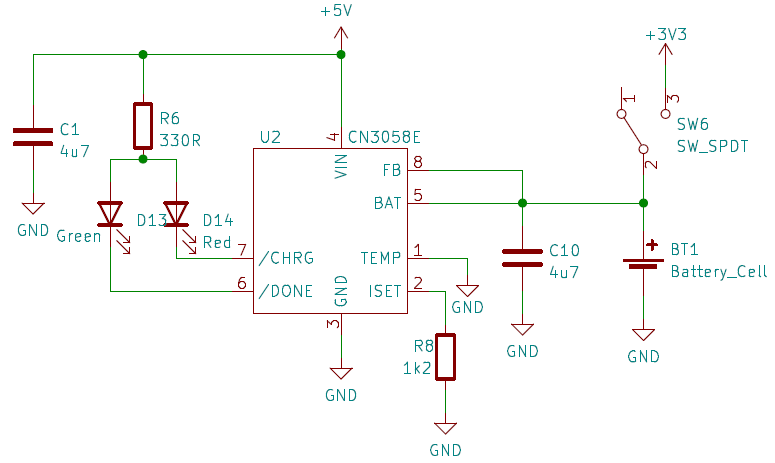
\includegraphics[scale=0.6]{obrazky/CN3058E.png}
  \end{center}
  \caption[Schéma zapojení nabíjecího obvodu pro LiFePO4]{Schéma zapojení nabíjecího obvodu pro LiFePO4.}
\end{figure}

\section{Senzory doteku}
V~návrhu Semaforu byla zvolena kapacitní dotyková tlačítka. Pro možnost použití uvnitř i venku jsou díky možnosti voděodolnosti 
vhodnějším řešením. Také velikost a označení tlačítka může být variabilní. Velikost může být na DPS navržena dle potřeby a potisk
v~místě tlačítka vyznačen barevně, nebo např. samolepkou. Odezva na dotyk bude realizována pomocí vibračního motoru.

\section{Vibrační motor}
Vibrační motory jsou založeny na principu kmitání. Motor je připevněn k~zařízení, které je kmitáním rozvibrováno. Vibrační motory jsou dnes 
nedílnou součástí mnoha elektronických zařízení včetně mobilního telefonu nebo dětských hraček. 

Dioda slouží jako ochrana proti přepětí, protože motor je indukční zátěž, takže vytváří napěťové špičky. Díky diodě je mikrokontrolér chráněn 
proti špičkovému napětí, které by se na něj mohlo dostat. Kondenzátor slouží k~tomu, aby napěťové špičky eliminoval, nebo alespoň zmenšoval. 

Vibrační motor je připojen k~mikrokontroléru přes tranzistor, protože maximální výstupní proud z~pinu MCU není dostatečně velký na to, aby 
motor roztočil. Tranzistor je tedy připojen na gate tranzistoru, který se při logické jedničce na pinu sepne a motorem protéká proud, který 
nedodává MCU, ale zdroj 3.3 V~(v~tomto případě baterie LiFePO4). Baterie tak dokáže dodat dostatek proudu, aby se motor roztočil. 

Pro Semafor byl vybrán vibrační motor LCM1020A2945F. Tento motor má maximální požadovaný proud 120 mA \cite{vib_motor_dtsh}. Maximální proud, 
který lze odebírat z~pinu mikrokontroléru ESP32-C3, je 40 mA \cite{ESP_C3_dtsh}. Vibrační motor lze pouze spínat, nebo je možné jej připojit 
k~pinu, který dokáže generovat PWM a lze tím regulovat jeho otáčky. 

Vibrační motor slouží jako odezva na dotyk kapacitního tlačítka. 

\begin{figure}[!h]
  \begin{center}
    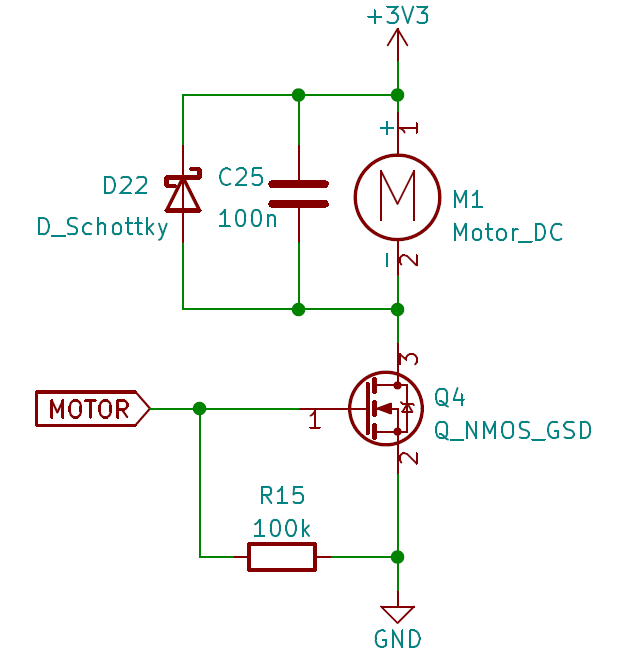
\includegraphics[scale=0.4]{obrazky/Vibracni_motor.png}
  \end{center}
  \caption[Schéma zapojení vibračního motoru]{Schéma zapojení vibračního motoru.}
\end{figure}

%fotka vybraného motoru

\section{Převodník pro kapacitní tlačítka}
Mikrokontrolér ESP32-C3 nemá kapacitní vstupy, proto je zapotřebí kapacitní dotyková tlačítka připojit přes převodník. Je zapotřebí připojit 
5 tlačítek. 

Vybraný převodník AT42QT1070 dokáže pracovat ve 2 režimech. V~prvním režimu může být zapojeno maximálně 5 kapacitních tlačítek, která jsou připojena
k~pinům KEY0 až KEY4. Jako výstup se používají piny OUT0 až OUT4. Každé tlačítko má tedy svůj výstup, který může být připojen k~GPIO pinům MCU 
nebo k~nim mohou být připojeny např. LED \cite{conv_cap_but_AT42QT1070_dtsh}. 

Druhý režim je využitelný pouze v~případě, je-li převodník připojen k~MCU. V~tomto případě může být k~převodníku připojeno až 7 kapacitních tlačítek, 
která jsou připojena na pinech KEY0 až KEY6. Převodník poté komunikuje s~MCU pomocí komunikační sběrnice $I^2C$ \cite{conv_cap_but_AT42QT1070_dtsh}. 
Z~registru převodníku lze poté vyčíst stavy daných kapacitních dotykových tlačítek. 

Jelikož je v~tomto návrhu Semaforu využit mikrokontrolér, který podporuje komunikaci po sběrnici $I^2C$, tak bylo využito zapojení právě s~tímto typem 
komunikace. Díky tomu budou využity pouze 2 GPIO piny mikrokontroléru ESP32-C3 a ne 5 GPIO pinů, které by byly zapotřebí při zapojení bez komunikace pro
sběrnici $I^2C$. Komunikační sběrnice $I^2C$ vyžaduje pullup rezistory, proto byly mezi napájecí napětí a piny SDA a SCL převodníku AT42QT1070 
přidány rezistory R17 a R18 o hodnotě 10 k$\Omega$. To znamená, že komunikační sběrnice $I^2C$ je aktivní v logické nule. 

Kapacitní tlačítka jsou připojena přes rezistory R19 až R23 k převodníku AT42QT1070. Tyto rezistory jsou připojeny sériově a slouží ke snížení šumu, 
omezení elektrostatických výbojů a potlačení radiofrekvenčního rušení \cite{conv_cap_but_AT42QT1070_dtsh}. Doporučená hodnota je rezistorů je mezi 
4,7k$\Omega$ a 20 k$\Omega$ \cite{conv_cap_but_AT42QT1070_dtsh}. Byla zvolena střední hodnota z doporučeného rozsahu, tj 10 k$\Omega$.

Převodník má kondenzátory C3 a C4 připojeny na napájecím pinu vůči GND, aby nebyly případné proudové špičky přivedeny na napájení převodníku. Rezistory
R17 a R18 slouží jako pullup rezistory při komunikaci pomocí sběrnice $I^2C$ s~mikrokontrolérem EP32-C3. Na piny KEY0 až KEY4 jsou připojena kapacitní 
dotyková tlačítka.  

Pin MODE je připojen k~signálu GND, protože převodník je provozován v~režimu komunikujícím přes $I^2C$ sběrnici \cite{conv_cap_but_AT42QT1070_dtsh}.

Pin /CHANGE je připojen k~GPIO pinu mikrokontroléru. Slouží pro indikaci změny stavu některého z~připojených tlačítek \cite{conv_cap_but_AT42QT1070_dtsh}. 
Signál z~tohoto pinu lze tedy využít jako indikátor vyvolání přerušení pro obsluhu tlačítek. 

\begin{figure}[!h]
    \begin{center}
      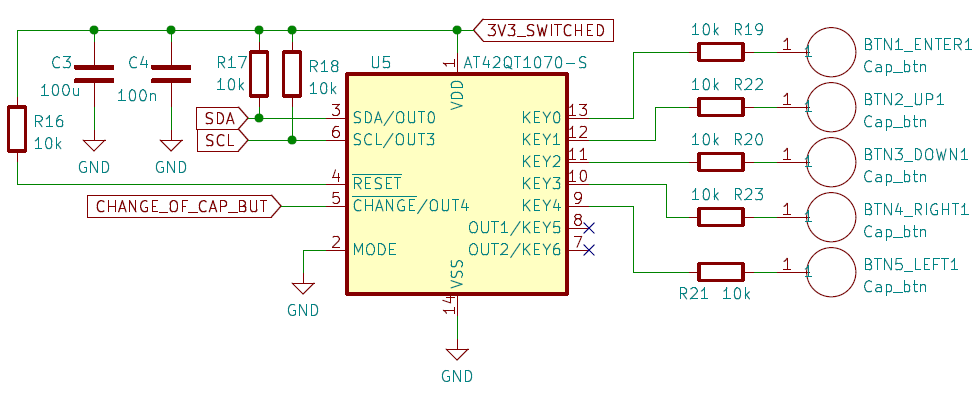
\includegraphics[scale=0.4]{obrazky/AT42QT1070.png}
    \end{center}
    \caption[Zapojení převodníku AT42QT1070 pro kapacitní tlačítka]{Zapojení převodníku AT42QT1070 pro kapacitní tlačítka.}
\end{figure}

\section{Světelná signalizace}
Pro realizaci signalizace přítomnosti napájecího napětí byly vybrány neprogramovatelné LED. Zelené LED byly vybrány dvě, jedna pro 
indikaci přítomnosti napětí 5~V a druhá pro indikaci přítomnosti napětí 3,3 V~z~baterií. Tyto LED budou použity pouze na prototypu 
pro ulehčení oživování. Dále budou odstraněny kvůli šetření energie, protože jde o~bateriově napájené zařízení. Přítomnost svitu 
tzv. power LED by také mohla mást při hře nebo různých úkolech.

Pro realizaci světelné signalizace pro hry byly vybrány inteligentní programovatelné LED typu WS2812C. Bylo jich použito 12, protože 
z~dvanácti LED lze jednoduše zhotovit ciferník pro odpočítávání času a také je lze rozdělit na segmenty na třetiny nebo čtvrtiny. 

Komunikační napěťová úroveň logické jedničky těchto LED by měla být alespoň na úrovni 70 \% napájecího napětí \cite{WS2812C_dtsh}. 
Protože použitý mikrokontrolér ESP32-C3 má komunikační napěťovou úroveň logické jedničky jeho napájecí napětí, což je 3 až 3,6 V, 
tak je zapotřebí využít převodník napěťové úrovně \cite{ESP_C3_dtsh}. Komunikace je v~tomto případě pouze jednosměrná, 
to znamená, že MCU posílá data do LED, ale LED neposílají žádná data do MCU. Převodník je realizován unipolárním tranzistorem 
a~jedním pullup rezistorem. Rezistor je připojen k~napájecímu napětí inteligentních LED WS2812C. 
Tranzistor Q1 má gate připojený k~napájecímu napětí MCU. Pokud bude mikrokontrolér do LED posílat logickou jedničku, tak bude rozdíl
mezi gate a~source 0 V. Tím pádem bude tranzistor uzavřený a tím se přes rezistor R4 připojí k~LED jejich napájecí napětí. Toto napětí 
je pro inteligentní LED logickou jedničkou. Pokud bude MCU posílat logickou nulu, tedy 0 V, tak je rozdíl napětí mezi gate a~source 
napájecí napětí mikrokontroléru. Tranzistor je tedy otevřený a tím se napětí 0 V~dostane k~inteligentním LED a na rezistoru se objeví
úbytek napětí o~velikosti napájecího napětí inteligentních LED. Napětí 0 V~je logickou nulou i pro inteligentní LED. Tento převodník
je určen pouze pro komunikaci jedním směrem. 

\begin{figure}[!h]
  \begin{center}
    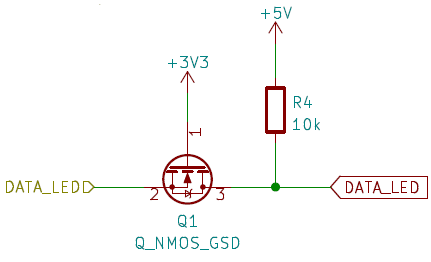
\includegraphics[scale=0.6]{obrazky/prevodnik_urovni_pro_WS2812C.png}
  \end{center}
  \caption[Zapojení převodníku úrovní pro WS2812C]{Zapojení převodníku úrovní pro WS2812C.}
\end{figure} 

\begin{figure}[!h]
  \begin{center}
    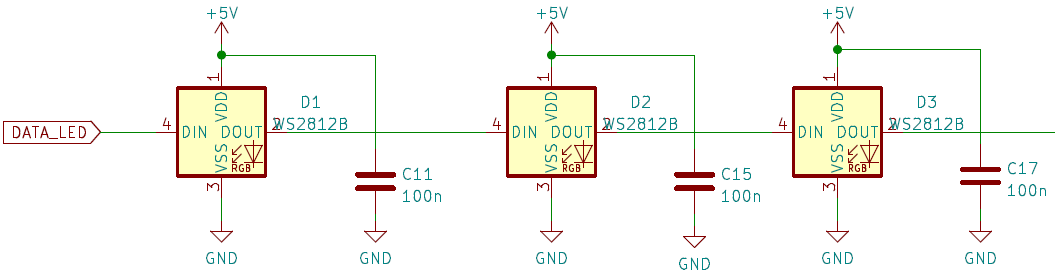
\includegraphics[scale=0.5]{obrazky/WS2812C.png}
  \end{center}
  \caption[Zapojení inteligentních LED WS2812C]{Zapojení inteligentních LED WS2812C.}
\end{figure}

Kondenzátor u~každé LED slouží pro filtraci napájecího napětí. 

Tyto programovatelné LED mají maximální spotřebu 5 mA na jeden kanál. Při zapnutí všech kanálů (svícení bílou) je maximální
spotřeba jedné LED 15 mA \cite{WS2812C_dtsh}. Pokud LED nesvítí, tak je její maximální klidový proud 0,3 mA \cite{WS2812C_dtsh}.
Při použití 12 LED je tedy maximální odběr všech LED 180 mA.

Pro napájení těchto inteligentních LED je zapotřebí napětí v~rozsahu 4,5 až 5,5~V \cite{WS2812C_dtsh}. 
Použité baterie LiFePO4 mají napětí pouze 3,2 V, proto je zapotřebí použít zvyšovač napětí na 5 V. 

\subsection{Zvyšovač napětí pro programovatelné LED}
Z~komerčně dostupných integrovaných obvodů byl hledán zvyšovač napětí, který vytváří z~napětí 3,3 V~napětí 5 V~a může přitom dodávat do výstupu proud alespoň 200 mA. 
Maximální odběr všech dvanácti potřebných inteligentní LED má maximální odběr 180 mA. S~rezervou je tedy zapotřebí proud alespoň 200 mA. Nalezené obvody, které vyhovují 
těmto parametrům jsou LT1930 a MCP1640. 

Obvod LT1930 v~doporučeném zapojení při vstupním napětí 3,3V vytváří výstupní napětí o~hodnotě 5 V~s~maximálním odběrem proudu 480 mA \cite{LT1930_dtsh}. Napájecí napětí 
tohoto obvodu je v~rozsahu 2,45 V~až 16 V, což vyhovuje napájecímu napětí z~baterií LiFePO4 \cite{LT1930_dtsh}.

Obvod MCP1640 v~doporučeném zapojení s~rozsahem vstupního napětí 3 až 4,2~V vytváří výstupní napětí o~hodnotě 5 V~s~maximálním odběrem proudu 300~mA \cite{MCP1640_dtsh}.

Byl vybrán zvyšovač napětí LT1930, díky své lepší dostupnosti v~této době nedostatku čipů, a také dokáže do výstupu dodat vyšší proud. Zapojení obou čipů je téměř totožné. 

Pin /SHDN slouží k~zapínání a vypínání obvodu. Pomocí přiloženého napětí 2,4 V~a více na tento pin je obvod zapnut \cite{LT1930_dtsh}. Pin SW slouží pro  připojení cívky, 
případně diody, aby se snížilo elektromagnetické rušení \cite{LT1930_dtsh}. 

Shottkyho dioda byla vybrána dle doporučení z~dokumentace. Byla vybrána dioda typu MBR0520, protože maximální napětí na diodě nepřekročí 20 V~a protékající proud nepřesáhne 
0,5 A~\cite{LT1930_dtsh}.

Byla vybrána cívka, která odpovídá doporučení z~dokumentace. Přesný typ, který byl v~dokumentaci zmíněn nebyl k~dispozici, a proto byl vybrán typ velmi podobný a vlastnostmi 
srovnatelný. Cívka CDRH3D18NP-4R7NC má feritové jádro, které je pro funkci požadováno \cite{LT1930_dtsh}. Pro typ LT1930 by měl být proud, který cívkou může protékat, alespoň
1A a její indukčnost by měla být 4,7 $\mu$H nebo 10 $\mu$H \cite{LT1930_dtsh}. Vybraná cívka má indukčnost 4,7 $\mu$H, proud, který jí může protékat, je 1,35 A~a její rozměry 
jsou 3,8 $\times$ 3,8 $\times$ 2 mm \cite{civka_dtsh}.

Pin FB slouží  pro zapojení zpětné vazby napětí na baterii. Jeho referenční napětí musí být nastaveno v~rozmezí 1,240~V až 1,270 V, typická hodnota je však 1,255~V \cite{LT1930_dtsh}. 
Pro výstupní napětí 5 V~byl zvolen rezistor R10 o~hodnotě 13 k$\Omega$ z~rezistorové řady E24 \cite{rezistorova_rada}. Řada E24 byla zvolena kvůli požadované přesnosti
napětí na pinu FB obvodu LT1930. Napětí na rezistoru R10 musí být tedy 1.255 V. Na rezistoru R9 je tedy úbytek napětí 3,745 V. Pomocí trojčlenky byla dopočítána hodnota 
rezistoru R9 dle rovnice:
\begin{equation} 
  R_{9}~=~\frac{R_{10}~\cdot~U_{R9}}{U_{R10}}~=~\frac{13~\cdot~3,745}{1,255}~=~38,79~\:k\Omega. 
  \quad
\label{eq:R9}
\end{equation}

Nejbližší hodnota rezistoru z~rezistorové řady E24 je 39 k$\Omega$ \cite{rezistorova_rada}. Reálná hodnota napětí na rezistoru R10, tj. napětí na pinu FB byla dopočítána
dle rovnice:
\begin{equation} 
  U_{R10}~=~\frac{U_{OUT}}{R_{9}~+~R_{10}}~\cdot~R_{10}~=~\frac{5}{39~+~13}~\cdot~13~=~1,25~V. 
  \quad
\label{eq:UR10}
\end{equation}

Napětí 1,25 V~je v~povoleném rozmezí napětí na pinu FB. 

Přesné výstupní napětí se spočítá podle vzorce:
\begin{equation} 
  U_{OUT}~=~U_{FB}~\cdot~(1~+~\frac{R_{9}}{R_{10}})~=~1,25~\cdot~(1~+~\frac{39}{13})~=~5~V. 
  \quad \quad \quad \quad \cite{LT1930_dtsh}
\label{eq:VOUT_LT1930}
\end{equation}

\begin{figure}[!h]
  \begin{center}
    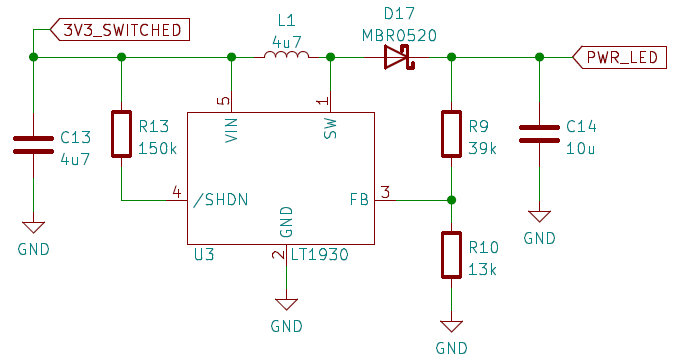
\includegraphics[scale=0.7]{obrazky/LT1930.png}
  \end{center}
  \caption[Zapojení zvyšovače napětí LT1930]{Zapojení zvyšovače napětí LT1930.}
\end{figure}

\section{Zvuková signalizace}
Zvuková signalizace může sloužit například pro potvrzení správnosti hesla, možnosti odejít na další stanoviště, vypršení času pro daný úkol a mnoho dalších. 

Jako zvuková signalizace bylo vybráno piezo s~vlastním oscilátorem typu \\BMT1205XH7.5 \cite{piezo_dtsh}. Maximální odebíraný proud vybraného pieza je 30 mA a rezonanční frekvence 
je 2,3 kHz \cite{piezo_dtsh}. Intenzita zvuku pieza je ve vzdálenosti 10 cm od něj minimálně 83 dB \cite{piezo_dtsh}.

\begin{figure}[!h]
  \begin{center}
    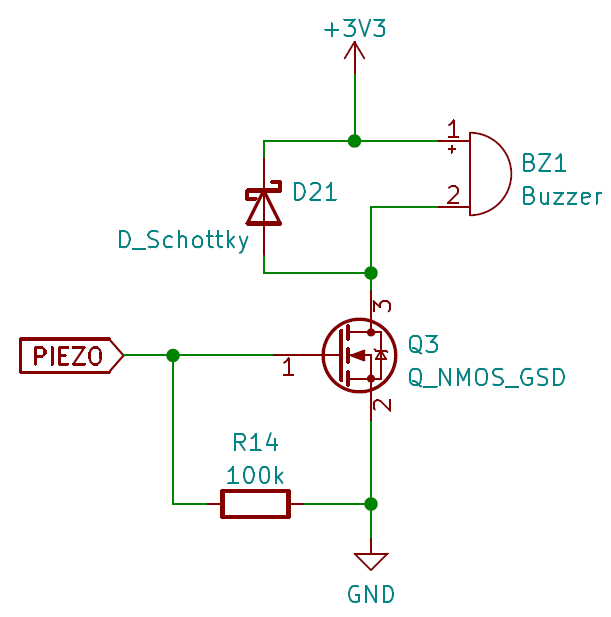
\includegraphics[scale=0.45]{obrazky/piezo.png}
  \end{center}
  \caption[Schéma zapojení pieza]{Schéma zapojení pieza.}
\end{figure}

\section{Konektor}
Jako programovací konektor byl zvolen konektor USB-C. Tento konektor je v~dnešní době velmi rozšířený a jeho použití se v~následující době stále rozšiřuje. 

Konektoru USB-C je využíván pouze jako standardní a dostupný konektor, který je mezi běžnou
populací rozšířený a v~následujících letech se bude rozšiřovat stále více. Je využito standardního jmenovitého napětí 5 V~pro nabíjení baterií a nadále pinů D+ a D-, 
které jsou využity pro komunikaci při programování. 

Konektor USB-C je robustní a oboustranný, díky čemuž nebude docházet k~tak častému poškození, jak by mohlo být např. u~konektoru Micro USB. Při používání běžnou veřejností
se jedná o~vítaný bonus. 

Vybraný mikrokontrolér ESP32-C3 umožňuje komunikaci přímo po USB protokolu a není díky tomu zapotřebí žádného převodníku pro komunikaci \cite{ESP_C3_dtsh}.

\begin{figure}[!h]
  \begin{center}
    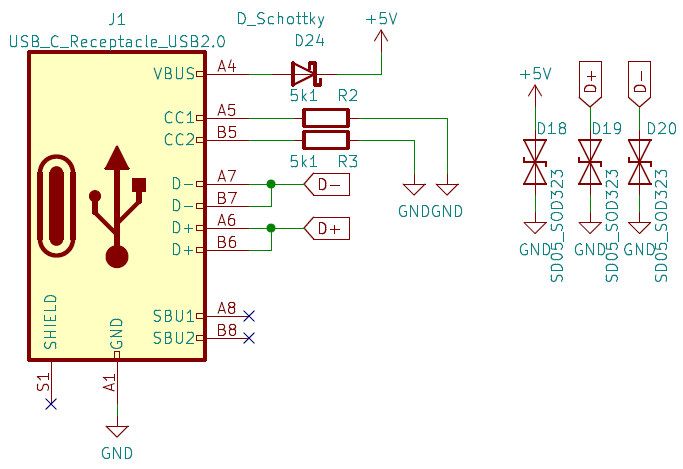
\includegraphics[scale=0.6]{obrazky/USB_C.png}
  \end{center}
  \caption[Zapojení konektoru USB-C]{Zapojení konektoru USB-C.}
\end{figure}

\begin{figure}[!h]
  \begin{center}
    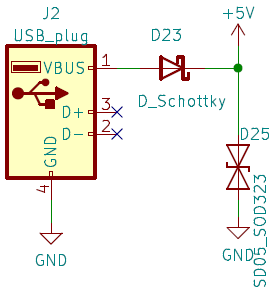
\includegraphics[scale=0.7]{obrazky/USB_A.png}
  \end{center}
  \caption[Zapojení konektoru USB-A]{Zapojení konektoru USB-A.}
\end{figure}

Připojené Shottkyho diody k~napájecímu napětí slouží pro zadržení případného zpětného proudu. Shottkyho diody jsou dimenzovány na proud, který odebírá celé zařízení. Vybrané 
Shottkyho diody  B5819W mají maximální napětí 20 V, jmenovitý proud 1 A~a maximální špičkový proud 9 A~\cite{shotky_dtsh}.

Transily připojené k~napájecímu pinu a ke komunikačním pinům D+ a D- slouží k~ochraně proti přepětí a elektrostatickým výbojům o~velikosti až 30 kV. 

Pro napájení pomocí powerbanky bez potřeby kabelu slouží konektor USB-A. 

Rezistory o~hodnotě 5,1 k$\Omega$ na pinech CC1 a CC2 slouží pro signalizaci, že je k~USB-C připojeno zařízení. Dle standardu USB-C totiž nabíječka bez 
připojení těchto rezistorů nesmí připojit napájecí napětí 5 V~na pin VBUS \cite{USB-C}. 

%ke každé komponentě napsat odběr

\section{Výsledné zapojení}
Pro realizaci Semaforu byly vybrány následující komponenty: mikrokontrolér ESP32-C3, baterie LiFePO4, nabíjecí obvod CN3056E, konektory USB-C a USB-A,
kapacitní tlačítka s~převodníkem AT42QT1070, inteligentní LED WS2812C s~převodníkem napětí LT1930, piezo, vibrační motor a LoRa modul. LoRa modul komunikuje 
s~mikrokontrolérem pomocí sběrnice UART, převodník pro kapacitní tlačítka pomocí sběrnice $I^2C$ a programování bude probíhat pomocí USB sběrnice. Vše je 
zapojeno dle následujícího blokového schématu. 

\begin{figure}[!h]
  \begin{center}
    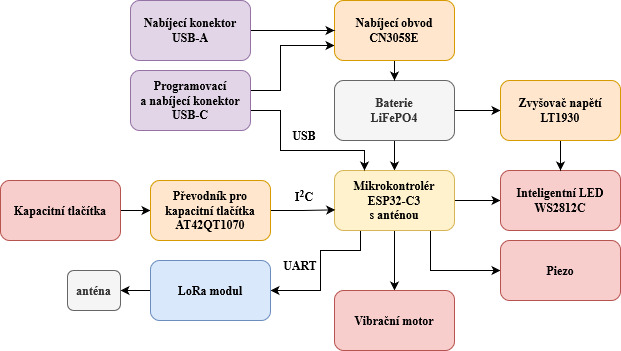
\includegraphics[scale=0.65]{obrazky/vysledne_blokove_schema.jpg}
  \end{center}
  \caption[Výsledné blokové schéma Semaforu]{Výsledné blokové schéma Semaforu.}
\end{figure}


\chapter{Návrh DPS}
Byl zvolen kruhový tvar desky s průměrem téměř 15 cm a s výběžkem USB-A pro připojení powerbanky. Deska plošného spoje byla navržena v programu KiCad 6.0 a má 2 vrstvy mědi. 
Některé součástky jsou natočeny tak, aby byly co nejvíce na kraji kulaté DPS.

Komunikační dráhy jsou vedeny o tloušťce 0,150 mm a napájecí dráhy jsou vedeny o tloušťce 0,5 mm. 

Výrobní podklady byly vygenerovány pomocí programu Kikit. Deska byla vyrobena u firmy JLCPCB, protože je bezkonkurenčně nejlevnější a její dodání je rychlé a bezproblémové. 
Jejich výrobky také dosahují vysoké kvality. 

\section{Kapacitní tlačítka} 
Byl požadavek na 5 tlačítek. Jedno tlačítko je uprostřed a slouží jako hlavní tlačítko. U her bude používáno např. jako registrace průchodu místem apod. Bude tedy nejčastěji
používáno a zároveň může být stisknuto, když hráč běží, takže by mělo být co nejjednodušeji stisknutelné. Proto bylo navrženo větší než zbylá tlačítka. Konkrétně má 
čtvercový tvar se zaoblenými rohy s rozměry 5~$\times$~5~cm. Ostatní tlačítka slouží například jako směrovky, nebo pro vyklikávání nějakého kódu, aby získali nějakou informaci. 
Slouží tedy primárně, když účastník u Semaforu stojí, nebo sedí, a vyklikává. Díky tomu mohou být tlačítka menší než hlavní tlačítko, konkrétně mají 2~$\times$~2~cm a jsou taktéž 
čtvercová se zaoblenými rohy. Tato tlačítka jsou proto umístěna po stranách hlavního tlačítka a jsou popsána BTN\_ENTER, BTN\_UP, BTN\_DOWN, BTN\_RIGHT a BTN\_LEFT.

V oblastech kapacitních tlačítek nejsou umístěny žádné další součástky a v jejich okolí je rozmístěna země kvůli odstínění. 

Pod spodním tlačítkem je ze spodní strany umístěno pouzdro na baterii. Kdyby bylo pouzdro až pod tlačítkem, musel by se ještě hodně zvětšit průměr DPS. Pokud by se při testování 
prototypu ukázalo, že kvůli umístění pouzdra baterie dochází k rušení tlačítka, tak dojde při výsledné verzi DPS k posunutí pouzdra baterie. 

\section{LED}
Po obvodu DPS je poté rovnoměrně rozmístěno do kruhu všech 12 programovatelných LED. Takto rozmístěné LED mohou zobrazovat např. podíl uběhnutého času. 12 LED bylo zvoleno z důvodu 
možnosti rozdělení na 2, 3 nebo i 4 segmenty. Na 12ti LED v kruhu lze také zobrazovat čas.

\section{Ostatní součáskty}
Ze zadní strany DPS je umístěna veškerá řídicí elektronika. Ve spodní straně je umístěno pouzdro s baterií LiFePO4 a v jeho blízkosti je umístěn nabíjecí obvod. V levém 
spodním rohu je poté umístěn konektor USB-C, který slouží pro nabíjení baterie a zároveň pro programování. Nad pouzdrem pro baterii je umístěn zvyšovač napětí pro programovatelné 
LED a nedaleko jsou LED diody indikující přítomnost napájecího napětí 3,3 V a 5 V. Ze zadní strany je v levé horní části umístěn mikrokontrolér ESP32-C3 a v pravé horní části 
LoRa modul. Nad tlačítky je umístěn převodník pro kapacitní tlačítka AT42QT1070-S.

Otvory pro připojení vypínače jsou umístěny u konektoru USB-C a otvory pro připojení vibračního motoru jsou umístěny mezi LoRa modulem a vrchním tlačítkem BTN2\_UP1. 

Z přední strany DPS je také umístěn bzučák. 

\section{Průběh návrhu}
Při návrhu DPS byla dodržována pravidla a dobré způsoby správného návrhu. %upravit tuto větu

V oblasti antény od ESP32-C3 mikrokontroléru nejsou taženy žádné dráhy, ani pod ní není rozlitá žádná měď. Je to z důvodu zaručení většího dosahu signálu a pro snížení rušení. 

Filtrační kondenzátory jsou vždy umístěny co nejblíže pouzdrům daných čipů. Shottkyho diody jsou umístěny v blízkosti USB konektorů. Rozmístění součástek kolem zvyšovače napětí 
je provedeno dle doporučení z dokumentace. 

Komunikační piny D+ a D- pro programování jsou taženy jako diferenciální pár.

\section{Osazení, oživení a testování DPS}
DPS byla taktéž strojově osazena u firmy JLCPCB. Z důvodu nedostupnosti některých součástek byly některé komponenty zakoupeny v jiných obchodních řetězcích a doosazeny ručně. 
Jednalo se o držák na baterie, piezo, kondenzátor C3 v pouzdře 0805 o hodnotě 100 $\mu$F, čip pro kapacitní tlačítka AT42QT1070, vypínač a LoRa modul. 

Nebyl sehnán přesný typ držáku, pro který byl modul navržen, proto byly nožičky držáku roztaženy, aby byla jejich rozteč zvětšena a mohlo dojít k zapájení. U pieza také chybělo 
označení polarity. Do finální verze bylo tedy přidáno do popisové vrstvy plus u správného vývodu. Vypínač byl kvůli testovacím účelům realizován pinheady a na ně byla nasazena 
propojka. Na místo LoRa modulu byly připájeny dutinky a LoRa modul byl pouze zasunut do dutinek. Hlavním důvodem byla cena tohoto modulu. LoRa modul bude z prototypu přesunut 
na finální výrobek a nedojde tak k plýtvání součástek ani peněz.

\subsection{Oživení}
Po připájení všech součástek byla do pouzdra vložena baterie LiFePO4 a DPS byla pomocí propojky zapnuta. Po zapnutí DPS se rozsvítila LED indikující přítomnost napětí 3,3 V. 
Po připojení konektoru USB-C s napájecím napětím se rozsvítila i LED indikující napětí 5 V. Také se rozsvítila červená LED indikující nabíjení baterie. Baterie byla pod dohledem 
nabíjena v DPS. Nedošlo k zahřátí DPS ani baterie a po čase se u nabíjecího obvodu rozsvítila místo červené LED zelená LED. Tato LED indikuje plně nabitou baterii. Na plně nabité 
baterii bylo naměřeno napětí 3,4 V. Nabíjecí obvod byl tedy otestován a bylo zjištěno, že funguje správně. 

Při měření napětí bylo zjištěno, že napájecí napětí pro programovatelné LED dosahuje pouze 1,7 V. Dalším měřením bylo zjištěno, že ani na vstupu zvyšovače napětí není 3,3 V, ale 
pouze 1,7 V. Díky tomu bylo zjištěno, že při logické 1 na pinu IO5 je 3,3 V, ale na spínaném výstupu je pouze 1,7 V. Bylo zjištěno, že byl použit tranzistor typu NMOS, který nelze 
v takovém zapojení plně otevřít. Tranzistor tedy zůstává v lineárním režimu, a proto je na výstupu pouze 1,7 V. Chyba byla vyřešena výměnou tranzistoru. Místo NMOS byl použit PMOS 
a do finální verze byla chyba opravena. Byla vyměněna schématická značka tranzistoru za PMOS a zároveň byl vyměněn kód součástky, aby byla správná součástka osazena již u firmy JLCPCB. 

Po opravě již mělo napájecí napětí pro inteligentní LED hodnotu 5 V. Díky tomu bylo zjištěno, že zvyšovač napětí funguje správně. 

\subsection{Testování}
DPS byla naprogramována a komunikace mezi počítačem a mikrokontrolérem proběhla bezproblémově. Byl napsán testovací SW pro programovatelné LED 
a další periferie. Díky tomu mohly být otestovány programovatelné LED. Všechny inteligentní LED bylo možné rozsvítit různými barvami, takže jsou plně funkční. Byla otestování funkčnost 
zapojení pieza a vibračního motoru. Obě zapojení byla funkční. 

Dále bylo testováno zapojení kapacitních tlačítek a jejich čtení. Pro komunikaci s čipem AT42QT1070 byla použita knihovna AtTouch, která je primárně určena pro Arduino \cite{AtTouch}. 
Knihovny pro Arduino bývají převážně s mikrokontroléry ESP32 kompatibilní. Nejdříve bylo zjištěno, že knihovna předpokládá připojení I2C na konkrétních pinech, tj. SCL na GPIO9 a SDA 
na GPIO8 \cite{AtTouch}. Mnou navržený modul má piny připojené naopak, tj. SCL na GPIO8 a SDA na GPIO9. Došlo tedy k upravení knihovny, aby jako vstupní parametry byly přebírány i GPIO 
piny I2C. Testovací software, který používal upravenou knihovnu AtTouch ale nebyl funkční. Nedocházelo k detekci stisku tlačítka a ani pin /CHANGE neměnil svůj stav. Ani po zapnutí 
softwarového pullup rezistoru nezačal pin /CHANGE generovat správné pulzy. Proto byla DPS 
připojena k osciloskopu. Nejdříve byla sledována komunikace po I2C pomocí pinů SCL a SDA. Díky tomu bylo zjištěno, že počáteční ustavovací komunikace probíhá v pořádku a mikrokontrolér 
se s čipem AT42QT1070 domluví. Díky tomu bylo zjištěno, že čip AT42QT1070 funguje správně, ale data jsou knihovnou AtTouch chybně zpracovávána. Tato knihovna také neumožňovala detekci 
stisků více tlačítek současně, i když tuto funkci použitý čip AT42QT1070 umí. Z tohoto důvodu bylo rozhodnuto, že bude mnou vytvořena nová knihovna, která bude tuto funkci podporovat 
a budou v ní odstraněny všechny chyby, které jsou v knihovně AtTouch. 

Při tvorbě knihovny bylo zapotřebí otestovat funkci jednotlivých registrů. Registr Detection Status generuje při doteku jakéhokoli tlačítka jedničku na bitu nula. Zároveň, pokud je tento 
registr čten, tak pin /CHANGE negeneruje pulzy a zůstává v klidové pozici, tj. logické jedničce. Bylo tedy rozhodnuto, že pokud se bude daná informace používat, tak to bude právě z registru 
Detection Status a díky tomu se uvolní pin na mikrokontroléru, který bude moci být použit pro připojení dalších periferií. Registr Key Status indikuje pouze stisk jednoho tlačítka. Pokud 
je jich stisknuto více, tak se celý vynuluje. Toto chování může být způsobeno velikostí kapacitních tlačítek, jejich návrhem, nebo může být chyba v čipu AT42QT1070. Registry Key Signal 
uchovávají aktuální měřenou informaci o měřené kapacitě ve 2 bytech pro každé tlačítko. Tyto hodnoty se mění v závislosti na prostředí, ve kterém se modul nachází, a také v závislosti 
na stisknu. Při stisku jsou hodnoty změněny skokově a hodnota měřené kapacity se výrazně změní. 
Registry Reference Data uchovávají data po kalibraci. Při testování se stávalo, že se kalibrace spouštěla sama ve chvílích, kdy bylo některé z tlačítek stisknuto. Zejména dělalo problémy hlavní
velké tlačítko. Proto byla v knihovně využívána data pouze z registrů Key Signal a změna byla detekována pouze pomocí tohoto registru. Díky tomu, že změna prostředí nedělá tak velké a prudké 
změny. Tlačítka byla nadále rozdělena do jednotlivých skupin, aby mohl být detekován i multistisk. To bylo nastaveno v registrech AVE/AKS. Bity 0 a 1 byly nastaveny do nuly, což znamená, že 
tlačítka nejsou v žádné skupině, takže je každé samostatně. Pro používaná tlačítka 0 až 4 byly nastaveny registry na hodnotu 32, což znamená, že měřená hodnota je průměrem z 8mi naměřených
hodnot. Registry pro tlačítka 5 a 6 jsou vynulovány, a tím jsou tyto vstupy deaktivovány. 

Pro práci s kapacitními tlačítky jsou tedy primárně využívány registry Key Signal a informace o stisku jsou z nich dopočítávány. 

Byla otestována komunikace s E22-900T22D LoRa modulem. Vyčítání informací z LoRa modulu probíhalo v pořádku, ale kvůli nepřipojení pinů M0, M1 a AUX k mikrokontroléru nemohl být modul nastaven
tak, aby komunikoval s dalšími moduly. Tyto chyby byly opraveny do finální verze a další testování tohoto modulu probíhalo až na hardwaru finální verze DPS. 
%testování LoRa modulu

\chapter{Finální verze DPS}
Finální verze DPS byla zmenšena na průměr 10 cm, protože DPS od firmy JLCPCB jsou mnohem levnější, když mají maximální rozměry 10$\times$10 cm. Také jejich skladovací nároky jsou mnohem  menší. 
Kvůli tomuto zmenšení ale nebylo dost místa 
kolem kapacitních tlačítek, aby nedocházelo k jejich rušení z okolních obvodů. Zároveň by musely být tlačítka moc blízko u sebe, takže by mohlo docházet k jejich přeslechům. Routování takové 
DPS, aby dráhy nevedly v blízkosti kapacitních tlačítek ani pod nimi bylo takřka nemožné. Proto bylo přistoupeno k řešení 2 spojených DPS. Díky tomu mohly být obě DPS osazeny pouze z jedné strany,
což ušetří další nemalé peníze. I při výrobě 2 kusů DPS o průměru 10 cm místo jedné velké byla cena výhodnější. Na spodní DPS je tedy veškerá řídicí elektronika a na vrchní DPS jsou pouze tlačítka 
a programovatelné LED. Kolem kapacitních tlačítek byla také vytvořena tzv. "guard" zóna, která slouží pro lepší odstínění tlačítek od ostatních signálů. Tato zóna byla připojena k převodníku AT42QT1070 
dle datasheetu na pozici prvního tlačítka - pin KEY0 \cite{conv_cap_but_AT42QT1070_dtsh}. 

Po konzultaci bylo domluveno, že při napájení z baterie a možnosti napájení přes konektor USB-C není konektor USB-A zapotřebí. Rozměry DPS by se tím také opět zvětšily a výrobní náklady by tím 
stouply. 

Do finální verze byl také přidán fototranzistor, který bude následně využíván pro regulaci jasu programovatelných LED typu WS2812C. Fototranzistor byl připojen na GPIO01 mikrokontroléru ESP32-C3. Na tomto 
pinu je k dispozici AD převodník \cite{ESP_C3_dtsh}. Byl vybrán fototranzistor s označením SMD3528C-50, který je citlivý na viditelné světlo. %citace https://jlcpcb.com/partdetail/Senba_SensingTech-SMD3528C50/C250859
Tento fototranzistor byl umístěn také na vrchní DP. Dále byl také 
přidán konektor pro připojení dalších programovatelných LED typu WS2812C, které budou na pásku, který bude připevněn po obvodu univerzálního modulu. Tyto LED budou zajišťovat, aby modul mohl svítit 
nejen dopředu, ale i do stran. Tato funkcionalita opět rozšiřuje možnosti využití tohoto modulu. Na datový pin těchto programovatelných LED byl připojen do série rezistor, který zabraňuje zničení pinu 
mikrokontroléru EPS32-C3, kdyby byly omylem zkratován s napájecím napětí. 

Bylo zapotřebí připojit k mikrokontroléru i piny M0, M1 a AUX od LoRa modulu E22-900T22D. Na mikrokontroléru ale nebylo již dostatek volných pinů a tak byl použit expander GPIO pinů. Vybraný expander
PCA9536D umožňuje připojení 4 GPIO a zároveň komunikuje s mikrokontrolérem přes sběrnici $I^2C$. Pin AUX byl tedy připojen k mikrokontroléru přímo přes GPIO05 a piny M0 a M1 byly připojeny k GPIO0 
a GPIO1 expanderu. Protože byly ještě volné GPIO piny na expanderu, bylo realizováno ještě samostatné vypínání napájení programovatelných LED, protože i když tyto LED nesvítí, tak mají stále spotřebu 
0,3 mA na jednu LED \cite{WS2812C_dtsh}. při bateriově napájení aplikaci je to stále nemalý proud, a proto byl realizován právě samostatný vypínač napájení. 
%citace expanderu PCA9536D

Ve finální verzi DPS byl použit posuvný vypínač se zahnutými vývody. Díky tomu mohl být vypínač umístěn na okraj DPS a nemusel být ručně pájen na drátkách. LED indikující přítomnost napájecího napětí 
3,3 V a LED indikující nabíjení nebo plné nabití baterie byly dány na okraj spodní DPS tak, aby bylo možné je vidět, ale zároveň aby při používání modulu při hře nemohly zmást. LED indikující přítomnost 
napájecího napětí 5 V byla odstraněna pro její nadbytečnost. 

Byly přidány také zkratovací prokovy na EN pinu mikrokontroléru s GND. Při zkratování je restartován mikrokontrolér. Tyto prokovy slouží pro snazší oživování a testování softwaru. Při proovozu nebude propojka 
zkratována a bude zabráněno jejímu náhodnomu zkratování díky obalu. 

Při návrhu byly také brány v potaz tekoucí proudy danými drahami. Tloušťky drah tomu byly přizpůsobeny a případné prokovy také. Například dráhy od baterie, jak k nabíjecímu obvodu, tak k USB mají tloušťku
2 mm, signálové dráhy mají tloušťku 0,125 mm a ostatní napájení dráhy mají tloušťku 1 mm. Prokovy mají vždy vrtanou díru stejně velkou, jako je tloušťka dráhy a okolní měď má průměr alespoň o 0,2 mm větší 
než vrtaná díra. U dvounožičkových součástek byl také řešen thombstone efekt. Proto u takových součástek byly dráhy vyvedeny stejně tlusté, případně alespoň co nejpodobnější. 
%obrázek řešení thombsone efektu - původní a řešení 

Rozložení součástek zvyšovače napětí bylo realizováno dle doporučení z datasheetu. Prokovy k signálu GND byly umístěny co nejblíže k vstupnímu i výstupnímu kondenzátoru. Propojovací konektory byly 
umístěny po obvodu a byly na ně připojeny všechny potřebné signály. Napájecí napětí a GND signál byly přivedeny přes jeden konektor, aby se tak zlepšilo EMC. 

DPS byla následně opět vyrobena a osazena u firmy JLCPCB. 
%propojení DPS realizováno prodlouženými pinheady, aby se mezi DPS vešla baterie. 
%napsat co jsem ručně osazovala
%napsat i oživení 

\chapter{Firmware}
V následující kapitole je popsán firmware univerzálního modulu. Jsou zde popsány veškeré vytvořené funkce a moduly, které jsou potřebné pro následnou tvorbu softwaru univerzálního modulu. 
%napěti 936 mV pri plnem napeti baterie
%napsat odpojovani napeti pri nizkem napeti baterie

%popsat celkovou funkci - vývojový diagram

\section{Tvorba hlavní knihovny}
Hlavní knihovna lib.h a lib.cpp slouží pro sdružování veškerých funkcí, které jsou univerzálnímu modulu k dispozici. Funkce init slouží pro počáteční inicializaci univerzálního modulu. Jsou zde 
zadefinovány piny mikrokontroléru, zda jsou vstupní, nebo výstupní, případně je zapnut softwarový pullup rezistor. Jsou zde nastaveny počáteční hodnoty výstupních pinů, vypnut vibrační motor, vypnuto 
piezo a zhasnuty všechny programovatelné LED. Jsou zde také vytvořeny všechny potřebné objekty, jako jsou tlačítka a programovatelné LED. 

Pro programování LED byla využita již existující knihovna Adafruit\_NeoPixel.h. Nad touto knihovnou byly vytvořeny nádstavbové funkce, aby práce s programovatelnými LED byla ještě snazší. 
Pro práci s programovatelnými LED byly vytvořeny následující funkce. Funkce set\_brightness vyčítá hodnotu z fototranzistoru a dle ní nastavuje jas programovatelných LED. Funkce colors přebírá jako
parametr název barvy a ten převádí do RBG kódu, se kterým již knihovna NeoPixel umí pracovat. Funkce get\_color přebírá jako parametr index LED a vrací barvu, kterou daná LED aktuálně svítí. 
Pomocí funkce LED\_light, která přebírá jako parametr index LED a barvu, lze rozsvítit LED na dané pozici danou barvou. Funkce LED\_toggle při každém volání funkce přepíná barvu LED mezi zadanou barvou 
a zhasnutím LED. Tato funkce přebírá jako parametr právě barvu, kterou má blikat a pozici LED, která má blikat. Funkce LED\_off zhasne LED na pozici, která je předána parametrem. Pro usnadnění práce 
se všemi LED yly vytvořeny také funkce LEDs\_all\_off, která zhasne všechny LED, LEDs\_all\_on, která přebírá jako parametr barvu a tou barvou poté rozsvítí všechny LED, a LEDs\_all\_toggle, která přebírá 
jako parametr barvu, kterou blikají všechny LED. Přepínání zhasnutí LED a rozsvícení danou barvou probíhá při každém zavolání této funkce. 

%zacházení s tlačítky 
%piezo
%motor
%LoRa
Pro hlídání stavu nabití baterií byly vytořeny 2 funkce. První funkce measure\_battery\_voltage měří napětí na baterie ve voltech, tato hodnota je také návratovou hodnotou této funkce. Druhou funkcí je 
is\_battery\_voltage\_ok, která vrací informaci, zda je baterie dostatečně nabitá. Pokud by vrátila informaci, že baterie je málo nabitá, tak na tento stav může program reagovat. Například je vytvořena 
funkce switch\_off\_voltage\_periferies, která odpojí od napětí periferie, které mají vyšší spotřebu. Jsou to například programovatelné LED nebo LoRa modul. 

\section{Knihovna pro AT42QT1070}
Pro převodník AT42QT1070, který převádí signál z kapacitních tlačítek na komunikaci po sběrnici $I^2C$, byla připravena knihovna AT42QT1070.h. Tato knihovna obsahuje 3 třídy, které dopomáhají 
práci s tlačítky a usnadňují ji. 

Třída s názvem AT42QT1070Touch obsahuje funkci begin, která slouží pro nastavení čipu AT42QT1070, rozděluje tlačítka do jednotlivých skupin a dělá počáteční kalibraci. Z tohoto důvodu nesmí být při 
zapnutí modulu stisknuto žádné tlačítko. Pokud by tomu tak bylo, tak by se tlačítka chybně zkalibrovala a docházelo by tak k falešným stiskům. Funkce tick musí být volána pravidelně, aby docházelo 
k neustálé obnově dat a kalibraci tlačítek. Díky tomu nejsou vyvolány falešný stisky při změně prostředí, která může způsobovat pozvolnou změnu kapacity. Funkce get\_raw\_data\_btn berejako parametr 
index tlačítka a vrátí hodnotu kapacity tlačítka přímo z registru čipu AT42QT1070. Funkce is\_touched\_btn přebírá jako parametr index tlačítka a vrací informaci o tom, zda je tlačítko stisknuto 
či nikoli.  

Třída s názvem TouchButton reprezentuje tlačítko. V této třídě je definována funkce tick, která přebírá aktuální vzorek z tlačítka. Tento vzorek je porovnáván s průměrně naměřenou hodnotou. Pokud 
je aktuálně naměřená hodnota blízká průměrné hodnotě, tak je tento vzorek započítán do průměru. Pokud je aktuálně naměřená hodnota dostatečně rozdílná oproti předchozím průměru, tak je detekován stisk. 
Stisk je signalizován až ve chvíli, když je neměřen 3$\times$ za sebou. Díky tomu jsou vyloučeny falšené stisky, které mohou být vyvolány například okolním rušením.  

Třída s názvem MovingAverage slouží pro počítání klouzavého průměru z naměřených hodnot z tlačítek. Funkce push\_sample převezme naměřený vzorek a nahradí jím nejstarší vzorek, který je pro počítání 
průměru využit. Funkce setup přebírá 2 parametry. První parametr size určuje, z kolika posledních naměřených vzorků bude průměr počítán, a druhý parametr initial\_value udává první hodnoty, které 
jsou po spuštění využity pro počítání průměru. Při použití jsou poté předávány hodnoty z počáteční kalibrace. 

\section{Webový server}

%pak upravit, podle skutečnosti
Pro práci s WiFi byla vybrána knihovna WiFi.h, která je určena pro Arduino i mikrokontroléry typu ESP32 \cite{WiFi_lib}. Testovací kód obsahoval vytvoření WiFi sítě a následně vytvoření webové 
stránky.  Telefon byl připojen k vytvořené WiFi síti a poté byl přesměrován na vytvořenou webovou stránku. Dále probíhalo testování získávání dat z nastavení na webové stránce. 


\chapter{Hry a jejich metodika}

\section{Odpočítávadlo}
%o hře - k čemu je možno využít
\underline{Funkce Semaforu ve hře:}

V konfiguraci je nastavena délka časového limitu. Poté je vysvícena dvanáctina času, který zbývá do konce časového limitu. Stisknutím prostředního tlačítka je odpočet zastaven. 
Zastavení času je signalizováno blikáním daného počtu LED červenou barvou. Opětovným stiskem prostředního tlačítka odpočet pokračuje. 

\section{Vábnička}
%o hře
\underline{Funkce Semaforu ve hře:}

Hru Vábnička lze hrát ve třech režimech. Nastavení režimu probíhá v konfiguračním menu. 

Režimy hry Vábnička: 
\begin{itemize} 
  \item Boční tlačítka mají charakter barev jednotlivých týmů. Po zmáčknutí daného tlačítka se Semafor rozsvítí danou barvou. 
  \item Středové tlačítko slouží pro přepnutí barvy na náhodnou jinou barvu, než kterou Semafor svítil do teď.  
  \item Středové tlačítko slouží pro přepnutí barvy na následující barvu, která je aktuálně v pořadí. 
\end{itemize}	
V konfiguraci lze také zapnout probíhání kontroly, aby jednotlivé Semafory nikdy nesvítily všechny stejnou barvou. Alespoň jeden Semafor musí svítit jinou barvou než ostatní. 
K tomu slouží komunikace mezi jednotlivými Semafory.

\section{Pán hory}
Hra Pán hory spočívá v délce času, jak dlouho který tým na hoře panuje. Každý tým musí doběhnout na horu a stisknout tlačítko svého týmu. Poté se počítá čas jeho týmu na úkor 
ostatních. Cílem je držet horu co nejdéle v rámci herního času. Hra je pro 2 až 4 týmy. 

Na počátku hry je čas všech týmů držení hory stejný. 

\underline{Funkce Semaforu ve hře:}

Jednotlivá boční tlačítka reprezentují barvy jednotlivých týmů a po stisku daného tlačítka se zahajuje přidávání času pro daný tým na úkor ostatních týmů. Kruh LED vždy svítí celý 
a barvy v něm jsou rozděleny právě v poměru časů držení hory daných týmů. Středové tlačítko slouží pro zastavení času. Žádný tým se nikam neposouvá. Boční LED slouží pro zobrazení 
barvy týmu, který je aktuálně pánem hory. Počet týmů je nastavován v konfiguračním menu. 

\section{Semafor}
Jde o naprogramování funkce klasického dopravního semaforu. 

\underline{Funkce Semaforu ve hře:}
Kruh je rozdělen na třetiny a každá třetina svítí jednou z barev klasického dopravního semaforu. Délka trvání jednotlivých stavů je náhodná v rozsahu 10 – 60 sekund. 


\chapter{Software}
%konkrétní hry 



\chapter{Voděodolnost}
Pro zajištění voděodolnosti byl zvolen obal z průhledného silikonu. Do silikonu je DPS zalita, proto musela být navržena forma pro následné odlití. V následující části je popsán postup 
návrhu formy a následná výroba silikonového pouzdra. Nejdříve byl celý proces otestován na prototypových DPS: Po odladění bylo vše překresleno podle finální verze DPS a byly zapouzdřeny
i finální verze univerzálního modulu.  

Nejprve byl vyexportován z programu KiCad 3D model celé DPS včetně všech součástek, které měly 3D model již z interní knihovny. Pro součástky, které neměly 3D model a zároveň byly důležité 
pro výsledný vzhled pouzdra, byly 3D modely dokresleny v programu SolidWorks. Pouzdra byly kresleny bez větších detailů. S přesností byly kresleny pouze kritická místa, kde součástka ovlivňuje 
rozměry pouzdra nebo kde musí procházet pouzdrem až na povrch.

%ukázka některého mnou kresleného pouzdra
%ukázka celé DPS

Náledně byl nakreslen model pouzdra, jak by mělo vypadat bez vložené DPS. Poté byla vytvořena sestava, kde byla DPS již vložené v pouzdře. Z pouzdra musely vyčnívat součásti, které nesmí být 
zality v silikonu. Nesmí být zalit USB konektor, prostřednictvím něhož je modul napájen a programován, dále vypínač a piezo, protože by jinak nemohlo vydávat zvuk. 
%ukázka DPS + obalu

Z takto vytvořeného modelu byla vytvořena forma. Byl nakreslen válec, který byl z každé strany o 3 mm větší než DPS s obalem. Poté byl použit nástroj "Kombinovat", který umožnil odečtení vytvořeného 
modelu DPS s obalem, takže vznikla dutá forma pro potřebný tvar. Následně byla forma rozdělena na 2 díly, které na sebe pasují a protínají v polovině všechny otvory tak, aby se do těchto půlek 
dala DPS zavřít.

Ve formě byl vytvořen otvor pro vstřik silikonu a také otvory pro XXX.

Forma na silikonový obal byla vytištěna na FMD 3D tiskárně. Nemohla být použita 3D tiskárna typu SLA, protože resin, ze kterého se v SLA tiskárnách tiskne, zabraňuje tuhnutí použitého typu silikonu. 

%jak udělat formu

%jaký typ silikonu je využit - na jaké bázi, jaké jsou jiné možnosti, výhody použitého typu 
Byl umíchán silikon z XXX v poměru 1:1. Pomocí stříkačky byl vtlačen silikon XXX. 
Tvrdnutí této silikonové směsy trvalo XXX. 
%fotka výsledného prototypu i s obalem



\chapter{Uživatelský manuál}
Po zapnutí Semaforu vypínačem je načtena poslední hraná hra. 

Po dobu XXX je možné přepnout modul do konfiguračního módu. Tento mód je k dispozici pomocí současného stisku tlačítek XXX. Konfigurační mód signalizován XXX. Po zapnutí tohoto módu je zapotřebí telefon 
nebo notebook, který má možnost připojit se k WiFi síti. V zařízení je zapotřebí najít WiFi síť s názvem XXX. Připojení proběhne po zadání hesla XXX. Po připojení k této WiFi síti přejďete do internetového 
vyhledávače. Do něj napište XXX. 

Zobrazí se webová stránka s konfiguračním menu modulu. Zde si můžete najít konkrétní hru i s jejím popisem. Pokud lze u dané hry nastavit nějaké parametry, jako je například počet hrajících týmů apod, tak 
jsou u této hry místa, kam lze daný parametr vyplnit. Pro nastavení dané hry stiskněte tlačítko dané hry. V tuto chvíli se spustí dané hra na nastavovaném modulu a zároveň na všech modulech, které jsou v danou
chvíli zapnuty a neuběhl u nich čas XXX od jejich zapnutí. 

Tímto způsobem lze konfigurovat až 9 modulů současně. 

Krátký popis funkce modulu v jednotlivých hrách je popsána na konfigurační webové stránce. 

\section{Funkce modulu v jednotlivých hrách}





